\documentclass[sigconf]{acmart}

\usepackage[ruled,algo2e]{algorithm2e}
\usepackage{algorithm}
\usepackage{hyperref}
\usepackage{bbold}
\usepackage{enumitem}
\usepackage{graphicx}
\usepackage{bm}
\usepackage{animate}
\begin{document}

\title{COMP6247 - Kalman and Particle Filters}
\author{Luke McClure \\ lam3g17@soton.ac.uk \\ 29573904}

\maketitle

\section{Time Varying AR - SIS/R}
\label{section:one}
By using Kalman Filtering we were able to learn the covariances within a time varying AR in order to forecast the sequence.\\

We can use sampling techniques to model the likelihood function without explicitly calculating covariances, this is useful in cases
where a likelihood function would be impossible to sample from directly and is the basis of SMCM methods Sequential Importance Sampling and Sequential Importance Resampling.

\subsection{Importance Sampling}
Importance Sampling relies on modelling a likelihood function using a number of weighted samples (particles), these weights dictate the likelihood an input at a timestep came from a specific particle via probability density functions.

This suffers with an issue known as weight degeneracy, where often one or two weights within the set will dominate. This results in a less accurate representation of the probability density function and so less accurate predictions.

\autoref{fig:WDSIS} shows the normalised magnitude of weights using the alpha value during a run of the SIS algorithm on a time varying AR problem. It is clear to see from how strong the colours present are that typically there is only a few particles being used at a given time step.

Effective Sample Size measures how many of the weights are in use by an importance sampling algorithm, the ESS accompanying this run is shown in \autoref{fig:ESS}.
\begin{figure}[h]
  \centering
  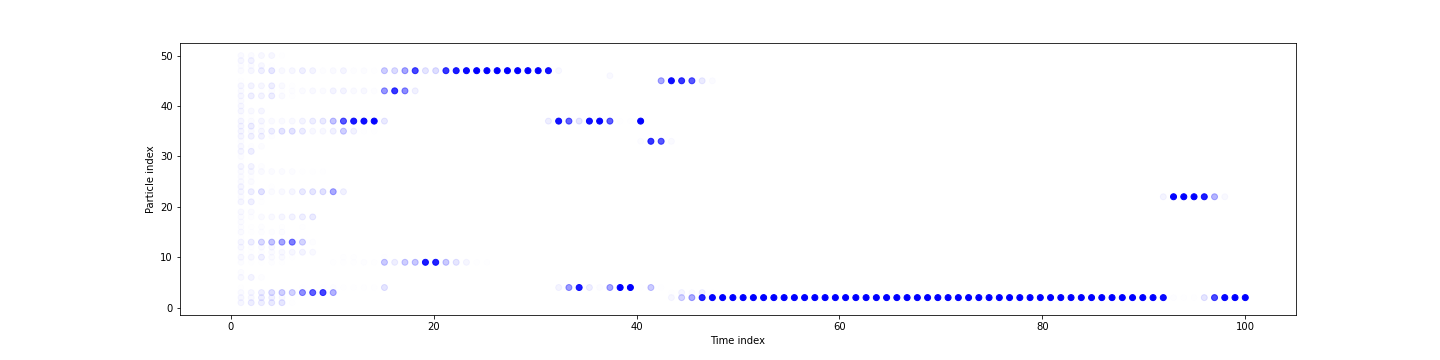
\includegraphics[width=\linewidth]{../Part 1/DegPlot.png}
  \caption{Weight Degredation using SIS}
  \label{fig:WDSIS}
\end{figure}

\subsection{Introducing Resampling}
Resampling allows the algorithm to choose particles that are more relevant to the problem and therefore replenish the samples and weights, this has the effect of focusing the particles sampled on to key areas and spreading what could have been one weight in SIS into a much wider proportion of the sample pool.

This combats weight degredation and improves on the accuracy of predictions the sampling algorithm is able to produce.

The normalised weight plot \autoref{fig:WDSIR} shows a stark difference when compared to \autoref{fig:WDSIS}. Weights in every timestep are significantly lighter in alpha signifying smaller weight values, spread throughout the entire sample pool so as to gather information from more particles. There are points such as at $t=58$ where these samples condense into a relatively smaller pool of larger weights before spreading back out again. 
\begin{figure}[h]
  \centering
  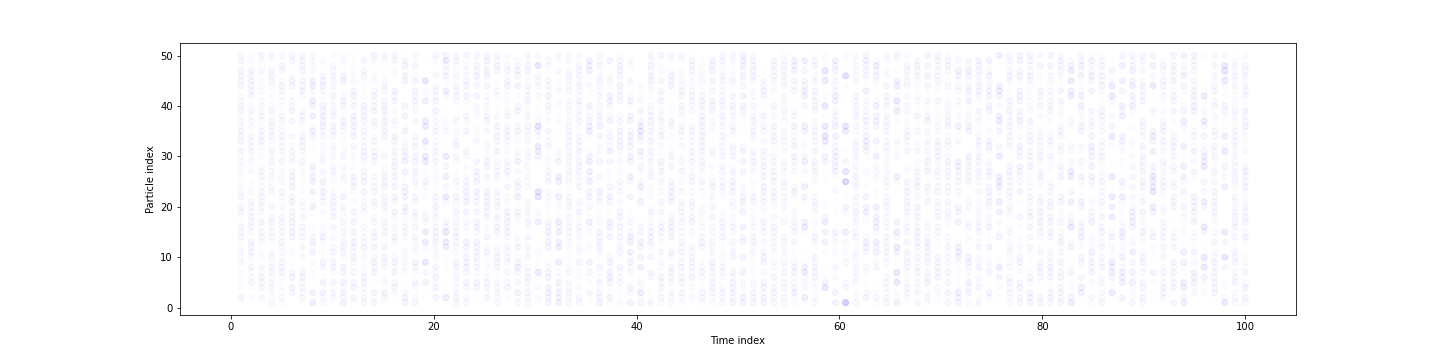
\includegraphics[width=\linewidth]{../Part 1/DegPlotResample.png}
  \caption{Weight Degredation using SIR}
  \label{fig:WDSIR}
\end{figure}

This is shown clearer when comparing the ESS of SIS with and without resampling in \autoref{fig:ESS}. The plot for SIS collapses quickly into using less than 5 weights while the SIR algorithm with resampling fluctuates but uses about 70\% of the available samples. The dips in sample size from \autoref{fig:WDSIR} are also clear in this plot, with several large dips in ESS.
\begin{figure}[h]
  \centering
  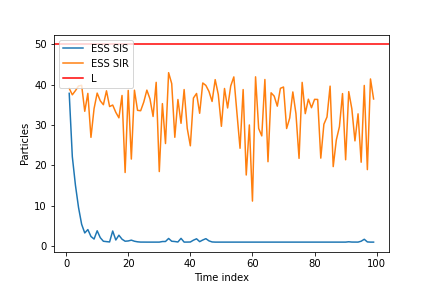
\includegraphics[scale=0.65]{../Part 1/ESSComp.png}
  \caption{ESS Comparison between SIS and SIR}
  \label{fig:ESS}
\end{figure}

\subsection{Comparing to Kalman Filter}
To compare these three methods, I have run each on the same Time Varying AR problem and have compared the predictive outputs in \autoref{fig:COMP}.
\begin{figure}[h]
  \centering
  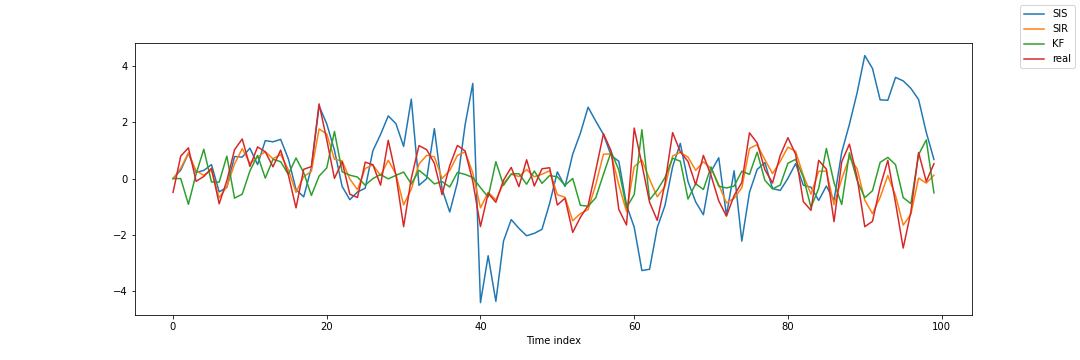
\includegraphics[width=\linewidth]{../Part 1/COMP.png}
  \caption{Prediction output of several methods}
  \label{fig:COMP}
\end{figure}
It is clear that Sequential importance Sampling performs the worst, with wild swings above and below the real value. It appears to be far more influenced by the momentum of the input, with these swings typically diverging at the peaks where it wildly overshoots instead of following the real inputs. This makes sense when thinking back to the weight degeneracy problem, if a trend occurs long enough to completely dominate the particle weights then it takes a while for the algorithm to recorrect, resulting in this overshooting behaviour.
Sequential Importance Resampling is the best performer of the three, tightly following the input. By resampling with every input allows the algorithm to keep an accurate track of the important particles and focus on these samples.
Karman filter was close to the performance of SIR, but appeared to lag behind the real inputs a little. This may be due to the time needed to update the covariance matrix estimation in a magnitude able to effect the predictions tangibly.

\begin{center}
  \begin{tabular}{||c c||} 
    \hline
    Method & MSE \\ [0.5ex] 
    \hline\hline
    Sequential Importance Sampling & 3.74 \\ 
    \hline
    Sequential Importance Resampling & 0.203 \\
    \hline
    Kalman Filter & 0.954 \\ [1ex] 
    \hline
  \end{tabular}
  \label{table:MSE}
\end{center}

There is a clear difference in performance between SIS and SIR, the resampling step is vital to keep the particles sampled relevant to the state of the input as well as the underlying process being modelled.
\section{Sequential Logistic Regression - Extended Kalman Filter}
\subsection{Algorithm}
In order to use Extended Kalman Filter to solve the sequential logistic regression problem, the portion of the kalman filter algorithm that preditcts $\theta$ needs to be changed such that it predicts the parameters of $$f(\bf{\theta}, \bf{x}) = \frac{1}{1 + \exp{(-\bf{\theta}^T\bf{x})}}$$
Achieving this so that EKF iteratively settles on the solutions for $\bf{\theta}$ given the known classes requires the derivative of $f$ wrt $\bf{\theta}$. $$f'(\bf{\theta}, \bf{x}) = f(\bf{\theta}, \bf{x})(1 - f(\bf{\theta}, \bf{x}))\bf{x}$$
As there are several dimensions to $\theta$, these derivatives form a 2x1 Jacobian matrix $H$.
\begin{algorithm2e}
  \caption{EKF algorithm update iteration solving Sequential Logistic Regression}
  \label{alg:EKF}
  \DontPrintSemicolon
  \KwIn{$x_t$,$z_t$,$\theta_{t-1|t-1}$,$P_{t-1|t-1}$}
  \KwOut{$\theta_{t|t}$,$P_{t|t}$}
  $P_{t|t-1} \gets P_{t-1|t-1} + Q$\;

  $y_t \gets f(\theta_{t-1|t-1}, x_t) $\;

  $e_t \gets z_t - y_t $\;

  $H_t \gets f'(\theta_{t-1|t-1}, x_t) $\;

  $k_t \gets \frac{P_{t|t-1}H_t}{H_{t}^{T}P_{t|t-1}H_t + R} $\;

  $\theta_{t|t} \gets \theta_{t|t-1} + k_t * e_t $\;

  $P_{t|t} \gets (I - k_{t}H^{T})P_{t|t-1}$\;
\end{algorithm2e}

\subsection{Solution Found}
\autoref{alg:EKF} was able to converge on the solutions displayed in \autoref{fig:EKFDBA}, how the algorithm settled on the decision boundary shown has been animated in \autoref{anim:EKF}.
\begin{figure}[!h]
  \begin{minipage}[b]{0.4\textwidth}
    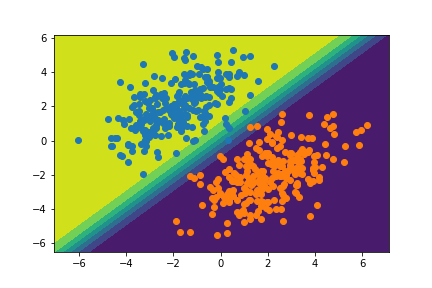
\includegraphics[scale=0.5]{../Part 2/DecisionBoundary1.png}
  \end{minipage}
  \hfill
  \begin{minipage}[b]{0.4\textwidth}
    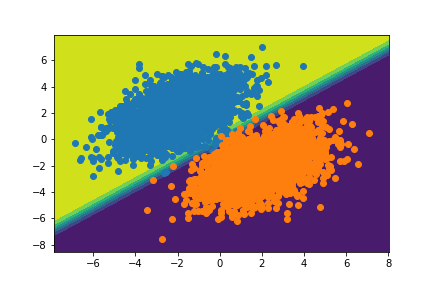
\includegraphics[scale=0.5]{../Part 2/DecisionBoundaryL.png}
  \end{minipage}
  \caption{Decision boundary found by EKF (L - 500 sample, R - 5000 samples)}
  \label{fig:EKFDBA}
\end{figure}

\begin{figure}[h]
  \centering
  \animategraphics[scale=0.5]{20}{../Part 2/imgs/frame_}{0}{499}
  \caption{EKF solving logistic regression (animation)}
  \label{anim:EKF}
\end{figure}

\subsection{Convergence}
The optimal solution for this problem is given by: $$w = \Sigma^{-1} (\mu_1 - \mu_2) $$ The EKF algorithm was rather slow in converging on this and didn't manage to within the 500 iterations given in \autoref{fig:EKFShort}.
\begin{figure}[h]
  \centering
  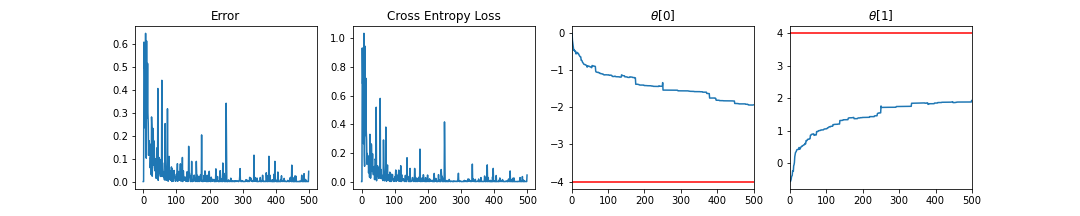
\includegraphics[width=\linewidth]{../Part 2/LogReg1.png}
  \caption{EKF to solve logistic regression}
  \label{fig:EKFShort}
\end{figure}

On further experimentation and running the algorithm with 5000 samples as shown in \autoref{fig:EKFLong}, the algorithm was much closer to the optimal convergence. The decision boundary found between the two runs is identical in gradient, with the only difference being the decision boundary is much narrower and well defined.
This reflects a greater confidence the algorithm has in the solution that has been found. \autoref{anim:EKF} reveals how the EKF algorithm is quick to settle near the optimal gradient of the boundary and simply gain confidence over time. 
\begin{figure}[h]
  \centering
  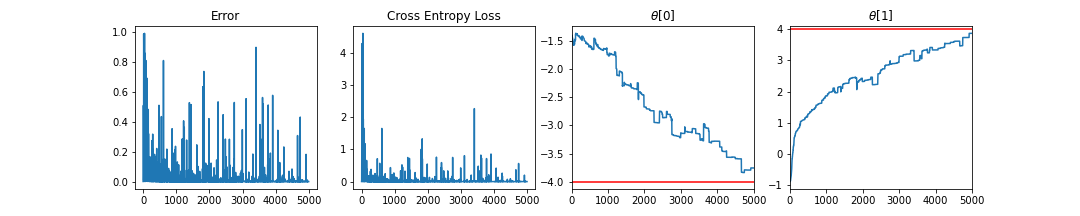
\includegraphics[width=\linewidth]{../Part 2/LogReg2.png}
  \caption{EKF to solve logistic regression (Extended)}
  \label{fig:EKFLong}
\end{figure}

\section{Sequential Logistic Regression - SIR}
\subsection{Algorithm}
Modifying the SIR algorithm from \autoref{section:one} follows much the same construct as modifying the KF algorithm into the EKF algorithm used earlier.
The same derivative of $f'(\bf{\theta}, \bf{x})$ will be used but instead in a diffent context in how it will be used as we cannot directly alter the covariances with an iterative error term. 
\\
There will be three key differences between standard particle filter used and the filter used for sequential logistic regression.
\begin{enumerate}
  \item We are going to use two separate particle filters to find the two dimensions of $\theta$.
  \item The probability density function for each dimension will use the respective dimension of $f'(\bf{\theta}, \bf{x})$.
  \item The input of the pdf will be the target of the logistic function at that input x.
\end{enumerate}

To solve this problem, the probability density function's mean is going to be centred on $H$, in doing so we will be placing the highest weights closer to $H$. 
By setting the mean to the derivative that is dependant on the input $x_t$ and $\theta$, and by setting the target of the probability density function to the correct output of the logistic function $y_t$, we are effectively setting up a likeness to the iterative error method that was seen in EKF.
This has the effect of steering the highest weighted particles towards the optimum of the derivative which happens to be $\theta$, which therefore will solve the logistic regression.

In implementation this may be split into two identical algorithms to be run concurrently for each timestep to deal with each dimension of $\theta_t$ and the sampling of $w_t$ more efficiently.

\begin{algorithm2e}
  \caption{SIR algorithm update iteration solving Sequential Logistic Regression}
  \label{alg:SIR}
  \DontPrintSemicolon
  \KwIn{$x_t$,$y_t$,$w_{t-1}$,$z_{t-1}$}
  \KwOut{$\theta_{t}$,$w_{t}$,,$z_{t}$}
  \KwData{$w_t : array, z_t : array$}
  $z_t \gets \mathcal{N}(z_t | \phi z_{t-1}, \sigma^{2}_{z}) $\;

  $\theta_{t} \gets w_{t-1} \cdot z_{t-1}$\;

  $H_t \gets f'(\theta_{t}, x_t) $\;

  $w_t \gets \mathcal{N}(y_t | \beta H_t, \sigma^{2}_{x})$\;

  $w_t \gets normalised(w_t) $\;

  $\theta_{t} \gets w_{t} \cdot z_{t}$\;

  $w_t, z_t \gets resample(w_t, z_t)$\;

\end{algorithm2e}

The algorithm relies on two 2xL sized arrays to hold the particles and weights to handle both particle filters being run concurrently, with L being the number of particles the algorithm will track. Python's ability to process entire arrays inplace allows for elegant processing in this manner during implementation rather than accessing every l of L in both arrays sequentially.
\subsection{Solution Found}
\autoref{alg:SIR} was able to converge on the solution displayed in \autoref{fig:SIRDB}, how the algorithm settled on the decision boundary shown has been animated on the right.

\begin{figure}[!h]
  \begin{minipage}[b]{0.4\textwidth}
    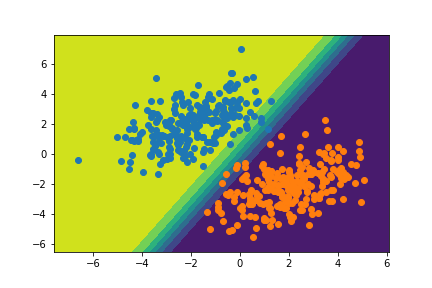
\includegraphics[scale=0.5]{../Part 3/DecisionBoundary.png}
  \end{minipage}
  \hfill
  \begin{minipage}[b]{0.4\textwidth}
    \animategraphics[scale=0.5]{20}{../Part 3/imgs/frame_}{0}{499}
  \end{minipage}
  \caption{SIR logistic regression (R - animation)}
  \label{fig:SIRDB}
\end{figure}

\subsection{Convergence}
It is clear to see from the animation in \autoref{fig:SIRDB} that \autoref{alg:SIR} is not as stable as \autoref{alg:EKF}. The animation shows the slope of the decision boundary wavering a lot compared to the animation of EKF, for a lot of the animation the decision boundary appears to stay close to parallel with the y axis, only starting to align with the proper decision boundary fairly late.

\begin{figure}[h]
  \centering
  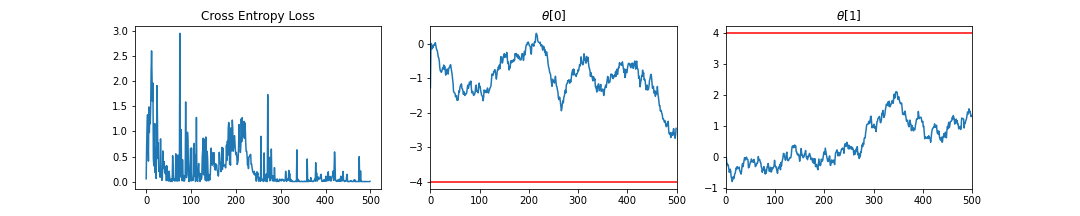
\includegraphics[scale=0.5]{../Part 3/SIRALL.png}
  \caption{SIR logistic regression}
  \label{fig:SIRALL}
\end{figure}

The plots in \autoref{fig:SIRALL} confirm this, showing that while the two parameters of $\theta$ do trend towards the optimal solution, there are plenty of periods where it is consistently heading away and the cross entropy loss is increasing.
In comparison, the results from \autoref{fig:EKFShort} and \autoref{fig:EKFLong} show that while there may be small periods of increasing cross entropy loss, EKF is a lot more reliable in converging on a solution and staying on it.

This is most likely due to the direct error comparison and derivative update being employed in EKF, rather than trying to pseudo recreate it with the mean of the probability density function. By directly altering the covariances rather than trying to target the weights close to the derivative creates a much more accurate and consistent update schedule for EKF compared to SIR.
\pagestyle{myheadings}
\end{document}
\endinput